% Two sided means the left and right margins are different sizes and they alternate every page. 
% If your document is printed to be book or spiral bound this allows for a thick spine to not 
% eat into the space for your page content. 
\documentclass[11pt, a4paper, twoside, openright]{custard}

% All imports, packages, and configuration in here. 
% Your document should be about content so we abstract away the styling rules and tools we are using. 
%% Here you can specify new commands and environments that you intend
%% to use. Using commands can make your document easier to write, read
%% and be more consistent.

\usepackage[linesnumbered,ruled]{algorithm2e}
\DeclareMathOperator*{\argmin}{arg\,min}

\usepackage{appendix}
\usepackage{textcomp}
\usepackage{setspace}
%\usepackage[document]{ragged2e}
\usepackage{verbatim}
\usepackage{multirow}
\usepackage{multicol}
\usepackage{booktabs}
\usepackage{enumitem}
\sloppy
\usepackage{graphicx}
\usepackage{threeparttable}
\usepackage{epsfig}
\usepackage{epstopdf}
\usepackage{float}
\usepackage{enumitem}
\usepackage{cite}
\usepackage[export]{adjustbox}
\usepackage{algorithmic}
\usepackage[nohyperlinks,printonlyused]{acronym}
\usepackage{amsmath}
\usepackage{amsfonts}
\usepackage{array}
\usepackage{tabularx}
\usepackage{longtable}
\usepackage{times}
\usepackage{amssymb}
\usepackage{hhline}
\usepackage{color}
\usepackage{soul}
\usepackage{colortbl}
\definecolor{Gray}{gray}{0.85}
\usepackage{rotating}
\usepackage{fix2col}
\usepackage{pdflscape}
\usepackage{pdfpages}
\usepackage{stmaryrd}
\usepackage[export]{adjustbox}
\usepackage{bbm}
\usepackage{relsize}
\usepackage{xfrac}
\usepackage{bibentry}

%\usepackage{refcheck}

%watermarking
\usepackage[english]{babel}
\usepackage{tikz}

%% Uncomment the following line for hyper links - not recommended for printing
\usepackage[colorlinks, linkcolor=, anchorcolor=, citecolor=, filecolor=, menucolor=, runcolor=, urlcolor=]{hyperref}

\setcounter{tocdepth}{1}
%\setcounter{minitocdepth}{3} 
\linespread{1.31}

\newcommand\litem[1]{\item{\bfseries #1:\enspace}}

\interdisplaylinepenalty=2500

\newcolumntype{L}[1]{>{\raggedright\let\newline\\\arraybackslash\hspace{0pt}}m{#1}}
\newcolumntype{C}[1]{>{\centering\let\newline\\\arraybackslash\hspace{0pt}}m{#1}}
\newcolumntype{R}[1]{>{\raggedleft\let\newline\\\arraybackslash\hspace{0pt}}m{#1}}

\renewcommand{\thefootnote}{\fnsymbol{footnote}}
\setlength{\LTpre}{-10pt}\setlength{\LTpost}{-30pt}%
\newcommand{\oiint}{\begin{picture}(0,0)(-10,-2)\put(0,0){\oval(12,8)}\end{picture}\iint}
\renewcommand{\mathbf }{\boldsymbol}

\def \eg{e.g.\ } % Allows you to write \eg in LaTeX instead of typing e.g. so that every single one will be formatted the same.
\def \Eg{E.g.\ } % Define some other common variants. If you later want to change one of these definitions, 
\def \ie{i.e.\ } % it will update all the usages throughout the document.
\def \Dr{Dr.\ }
\def \vs{vs. }
\def \etal{\emph{et al.\ }} 
\def \sota{state-of-the-art }
\def \handcrafted{hand-crafted }

\usepackage{listings,lstautogobble}
\usepackage{sourcecodepro}
\pdfmapfile{=SourceCodePro.map}
\lstset{
	xleftmargin=0.5cm,frame=tlbr,framesep=4pt,framerule=0.5pt,
	language=,
	upquote=true,
	columns=fixed,
	tabsize=2,
	extendedchars=true,
	breaklines=true,
	numbers=left,
	numbersep=10pt,
	basicstyle=\ttfamily\scriptsize,
	numberstyle=\tiny,
	stringstyle=\ttfamily,
	captionpos=b,
	showstringspaces=false,
	autogobble=true
}

\usepackage[font=small,skip=10pt]{caption} %,format=hang
%\usepackage[labelformat=simple]{subcaption}
\usepackage[labelformat=simple]{subfig}
%\captionsetup[figure]{format=hang}
%\captionsetup[lstlisting]{format=hang}
\renewcommand{\thesubfigure}{\Alph{subfigure}.}

\renewcommand{\thefootnote}{\arabic{footnote}}

% Use IEEEtran citation style. 
\bibliographystyle{IEEEtran} 

\def\samplefont#1{%
    % set font style and save name
    #1\edef\savedname{\fontname\font}%
    % print small sample
    {\leavevmode\tt\hbox to 1in{\savedname:\hss}}%
    abcxyz ABCXYZ 123\par
}

\begin{document}
	
% The custom data for Swansea University and your degree name.
% The \protect\\ command forces a new line in the title which might be otherwise overriden by the template
	\title{Safety Critical 2D Pen Plotter}
	\author{Arran Jones\protect\\{\normalsize 945187}}
	\awardinginst{Swansea University}
	
% Comment / uncomment your degree type as needed.
	%\degree{Bachelor of Science} 
	\degree{Master of Science}
	%\degree{Doctor of Philosophy}
	
% Institution details and logo
	\department{Department of Computer Science}
	\university{Swansea University}
	\unilogo{graphics/swansea.png}
	
% Hard code the date or allow the LaTeX compiler to fill it in whenever you recompile the document.
	\date{September 2020}
	
% Build the title and declaration pages, and pad the document so the text starts on a right hand book page.
% Page numbering is in roman numerals until the first page of an actual chapter which resets numbers 
% starting from 1 at that point. 
	\frontmatter%
	\maketitle
	\declaration
	\cleardoublepage
	
% Most books and theses have a brief foreword or dedication. 
%	\begin{vplace}[0.7]
%		\begin{large}
%			\begin{center}
%				\textit{I would like to dedicate this work to the Hypnotoad.\\All glory to the Hypnotoad.}
%			\end{center}
%		\end{large}
%	\end{vplace}

% Abstract comes before the contents page.	
	\begin{abstract}
		\vspace{-2em}
		\setcounter{page}{1}
		
		This document is a report on the progress and findings of a dissertation to implement a 2D pen plotter using safety critical design and implementation techniques. This project is split into 4 major sections. The conversion of DXF files into GCODE, the conversion of rasterized images (such as a PNG file) into GCODE, a simulator for a 2d pen plotter robot and a robust GUI for controlling the entire system. The original plan was to create a robot out of lego mindstorms which would move a pen around a sheet of paper to draw the product, but unfortunately COVID-19 caused the country to go into lockdown and obtaining the lego mindstorms kit became problematic. It was then that a simulator would be necessary to complete the project.
		
		This project will require rigorous testing, multiple fail-safes and emergency stop buttons for each section in order to produce a safe and reliable product. In order to ensure this is all complete on time, a strict time schedule will be required. This will be maintained by using a modified version of scrumban, where the idea of sprints will be implemented along side the time management systems of kanban. This will need to be modified as scrumban is usually used for a team of developers, whereas this will be a solo project.

	\end{abstract}
	
% A long form dedication. 
%	\begin{Acknowledgements}
%		This is an opportunity to acknowledge and thank those who have supported you throughout your studies. Friends and colleagues who you have studied alongside, your families, and your mentors within the department are the usual suspects. 
%	\end{Acknowledgements}
	
% Build the table of contents page.
	\tableofcontents*
	 
% Optionally you can make a bank of known acronyms in acronyms.tex that you can call on throughout your document.
	%\input{acronyms} 
	
% For long documents like a Doctoral thesis you should include a list of tables and figures throughout 
% your document. This is uses a shortened version of each table and figures caption and enumerates all 
% of them with their table or figure number. This is automatic, you do not need to modfy it if you do use it.
	\setlength{\columnsep}{10pt}
\newpage
\listoftables
\mtcaddchapter 
\newpage
\listoffigures
\mtcaddchapter  
	
% Reset numeric page numbering from page 1
	\mainmatter%

% Insert the code for each of your chapters
	\chapter{Sprint 1 - Background Research}
	\label{chap:background}
		
	Before starting the project a lot of background research was required, as there was no prior knowledge of GCODE, DXF files or safety critical systems. This chapter outlines researched topics required to gain enough understanding to begin the project and what was learnt during the research.

	\section{Safety Critical Systems}
		The first section which required research was safety critical systems. This was the main topic of the dissertation and there was no prior knowledge of the topic going into the project. This meant that a lot of prior research was required in order to ensure the system followed a safety critical level design, implementation and testing.
		
		
	\section{GCODE}
		\label{sec:gcode}

		The second topic that required research was GCODE

		The internet is big \cite{sizeofinternet}. Knowing how to phrase a question to a search engine is therefore an invaluable skill. If the request is simple enough, even a poorly structured query will likely return usable results. For more difficult to find resources you can leverage the language of the search engine to gather relevant papers and resources for your research more efficiently. 
		
		% An example of how to center a passage of text, control local fontsize, 
		% and create a properly formatted and clickable URL.
		\begin{center}
		{\small \url{https://www.gwern.net/Search}}
		\end{center}
		
		``Internet Search Tips'' \cite{gwern} provides an excellent review of methods and tips for scouring the internet for hard to find resources. You will also be less likely to get caught behind journal paywalls when working remotely without a tunnel as your queries can be made to look for raw pdfs that are often released by the authors directly.
			
	\section{Organizing your citations in BibTeX}       
		\label{sec:resources_bibtex}
	
		BibTeX is a language for specifying resource citations. Every time you access and read an academic paper, take code from an online repository, or source the media such as images from existing works you should create a BibTeX entry in a file that you keep throughout your research. Software such as Mendeley \cite{mendeley} can help automate the process of building your BibTeX library of citations. 
		
		\lstinputlisting[label={lst:bibtex}, caption={An example BibTeX entry for an academic paper published in conference proceedings \cite{kaj86}.}]{./listings/example_bibtex.bib}
		
		The BibTeX code listing above (listing \ref{lst:bibtex}) shows an example of how to cite an academic paper, in this case one of the central papers in Computer Graphics research. The key \textbf{kaj86} is an arbitrary name chosen as a meaningful identifier for the resource. In the document text we can call on this resource as an inline citation using the LaTeX command \lstinline|\cite{kaj86}| which produces \cite{kaj86} at the location it is called. As long as a citation has been used at least once somewhere within the document then a formatted full citation will be created in the bibliography at the end of the document with the same citation number that is shown inline.
		
		It is considerably easier to be disciplined in methodically taking note of the resources you access and make use of as you access them, than it is to try and hunt them all down again at the time you need to write about them in your document. Invest time in being organized and consistent up front and it will be easier when you come to write up.
		
	\section{DXF}
		Usually you would not put the URL of the resource you are citing directly in the text like is done previously in section \ref{sec:google_fu}. The citation for the resource \cite{gwern} is sufficient to reference it within the text given that full details of its location are then kept neatly within the bibliography at the end of the document. 
		
		In normal usage the purpose of a citation is not to direct the reader away from your thesis, but to justify and back up assertions you are making about the state of the domain. If a reader questions your assertions then they can follow the rabbit hole of papers which will likely also make and justify assertions with even earlier papers from the literature. 
		
		In the above case the intention is for the reader of this template to actually go to that resource and read what it has to say directly. The link is therefore shown clearly within the main text to indicate that the reader should visit it. This as opposed to wanting the reader to purely acknowledge that the facts which are within the resource legitimize the points made in this document, in which case a simple inline citation is the best way to back up your assertions. Section \ref{sec:typesetting_figures_citation} specifically touches on the best practice for how to cite images which you are importing from existing work. 
	\chapter{Sprint 2 - DXF to GCODE}
	\label{chap:background}
		
	After completing the background research, the first thing to be worked on was the conversion of a DXF file into basic GCODE instructions.

	\section{Safety Critical Systems}
		The first section which required research was safety critical systems. This was the main topic of the dissertation and there was no prior knowledge of the topic going into the project. This meant that a lot of prior research was required in order to ensure the system followed a safety critical level design, implementation and testing.

	\section{GCODE}
		\label{sec:google_fu}
		The internet is big \cite{sizeofinternet}. Knowing how to phrase a question to a search engine is therefore an invaluable skill. If the request is simple enough, even a poorly structured query will likely return usable results. For more difficult to find resources you can leverage the language of the search engine to gather relevant papers and resources for your research more efficiently. 
		
		% An example of how to center a passage of text, control local fontsize, 
		% and create a properly formatted and clickable URL.
		\begin{center}
		{\small \url{https://www.gwern.net/Search}}
		\end{center}
		
		``Internet Search Tips'' \cite{gwern} provides an excellent review of methods and tips for scouring the internet for hard to find resources. You will also be less likely to get caught behind journal paywalls when working remotely without a tunnel as your queries can be made to look for raw pdfs that are often released by the authors directly.
			
	\section{Organizing your citations in BibTeX}       
		\label{sec:resources_bibtex}
	
		BibTeX is a language for specifying resource citations. Every time you access and read an academic paper, take code from an online repository, or source the media such as images from existing works you should create a BibTeX entry in a file that you keep throughout your research. Software such as Mendeley \cite{mendeley} can help automate the process of building your BibTeX library of citations. 
		
		\lstinputlisting[label={lst:bibtex}, caption={An example BibTeX entry for an academic paper published in conference proceedings \cite{kaj86}.}]{./listings/example_bibtex.bib}
		
		The BibTeX code listing above (listing \ref{lst:bibtex}) shows an example of how to cite an academic paper, in this case one of the central papers in Computer Graphics research. The key \textbf{kaj86} is an arbitrary name chosen as a meaningful identifier for the resource. In the document text we can call on this resource as an inline citation using the LaTeX command \lstinline|\cite{kaj86}| which produces \cite{kaj86} at the location it is called. As long as a citation has been used at least once somewhere within the document then a formatted full citation will be created in the bibliography at the end of the document with the same citation number that is shown inline.
		
		It is considerably easier to be disciplined in methodically taking note of the resources you access and make use of as you access them, than it is to try and hunt them all down again at the time you need to write about them in your document. Invest time in being organized and consistent up front and it will be easier when you come to write up.
		
	\section{DXF}
		Usually you would not put the URL of the resource you are citing directly in the text like is done previously in section \ref{sec:google_fu}. The citation for the resource \cite{gwern} is sufficient to reference it within the text given that full details of its location are then kept neatly within the bibliography at the end of the document. 
		
		In normal usage the purpose of a citation is not to direct the reader away from your thesis, but to justify and back up assertions you are making about the state of the domain. If a reader questions your assertions then they can follow the rabbit hole of papers which will likely also make and justify assertions with even earlier papers from the literature. 
		
		In the above case the intention is for the reader of this template to actually go to that resource and read what it has to say directly. The link is therefore shown clearly within the main text to indicate that the reader should visit it. This as opposed to wanting the reader to purely acknowledge that the facts which are within the resource legitimize the points made in this document, in which case a simple inline citation is the best way to back up your assertions. Section \ref{sec:typesetting_figures_citation} specifically touches on the best practice for how to cite images which you are importing from existing work. 
	\chapter{Typesetting your thesis}
	\label{chap:typesetting}
	
	This document is intended as both a LaTeX thesis template and as a tutorial on structuring and typesetting your thesis in the LaTeX programming language.
	
	The following are some powerful online resources for learning about LaTeX:
	
	\begin{description}	
			
		\item[$\bullet$ Overleaf Documentation for LaTeX]\hfill
		
		Overleaf \cite{overleafdocs} is an online browser-based LaTeX IDE which stores your document in the cloud and provides live recompilation as you type. The documentation on Overleaf's website has a good knowledge base of examples for how to typeset things cleanly and simply in LaTeX code. 
		
		\noindent See: {\small \url{https://www.overleaf.com/learn}}
		
		\item[$\bullet$ TeX StackExchange, the StackOverflow site dedicated to TeX questions]\hfill
		
		TeX StackExchange \cite{texstackexchange} is sub-community of the StackOverflow network dedicated to questions about the TeX family of typesetting tools including LaTeX, BibTeX and others. A vast majority of the time it is unlikely that the question or issue you are facing is one that has not been encountered before, and this site more than likely to be able to point you in the correct direction. 
		
		\noindent See: {\small \url{https://tex.stackexchange.com}}
		
	\end{description}
	
	\newpage 
		
	\section{Referencing items within this document}
		In section \ref{sec:resources_bibtex} we saw examples of how to typeset citations for resources we had stored in an external BibTeX file. However, often we would like to accurately refer to the location of a resource or region of text stored somewhere else within this document\footnote{Like at the beginning of the last sentence when we referred to section \ref{sec:resources_bibtex}.}. To do this we need to annotate our LaTeX code with \lstinline|\label{key}| statements which will take on the numeric (or otherwise formatted) identifier for the current chapter, section, figure, table, equation, ect where they are directly defined. To insert an inline reference to the label you can use the \lstinline|\ref{key}| command which works similarly to the \lstinline|\cite{key}| used for external references. In the event we chose to reorder or add additional content to the document, which would change the section numbering, the document will still compile to a pdf with the correct references inserted for each \lstinline|\ref{key}| command.
		
	\section{Equations}
	\label{sec:typesetting_equations}
	
	Typesetting equations is one of the things that LaTeX does best. It has packages for different fonts and symbols for many different mathematical notations. However, to person learning how to typeset in LaTeX for the first time it can be a daunting and unwieldy user experience. Almost all LaTeX packages have documentation available in pdf format online, and documentation for packages specifically relating to fonts and symbols usually have tables enumerating the names and codes for all of the fonts symbols, organized by intended usage. 
	
	\subsection{Inline equations}
	
	Small equations like $x = 0$ can be written directly within the text by using LaTeX's maths mode shorthand controlled by dollar signs \lstinline|$ math mode $|. As long as it is not becoming cumbersome to the reader, equations such as $\mathbb{P}({A} \cap {B}) = \mathbb{P}({B} \cap {A})$ are quite neatly displayed in this fashion. 
	
	\newpage 
	
	\subsection{Block equations}
	
		For long equations it is best to provide a break in the main text of the document and format the equation using a \lstinline|\begin{equation}...\end{equation}| environment. 
		
		\begin{equation} \label{eq:veclen}
			\left\lvert a \right\rvert = \left\lvert \left[\begin{array}{c} a_0\\ a_1\\ \vdots\\ a_n\end{array}\right] \right\rvert = \sqrt{a_0^2 + a_1^2 + \hdots + a_n^2}
		\end{equation}
		
		Equation \ref{eq:veclen} demonstrates formatting a larger equation and uses an \lstinline|\begin{array}...\end{array}| environment to structure a column vector of sub-equations. Block equations should be located at a relevant point directly as they are being referred to in the text. When referred to from other locations in the document you should use the \lstinline|\ref{key}| command to insert the correct equation number.
		
		\subsubsection{Aligning multi-line block equations}
		
			When equations become even larger they may need cross over multiple new lines. When this happens it is desirable to align relevant parts of the equation on each line to one another for aesthetic reasons and to help imply structure to the reader. 
		
			\begin{equation} \label{eq:rendering_equation}
				\begin{split}
					\mathcal{L}_o\left(x, \omega_o, \lambda, t\right) &= \mathcal{L}_e\left(x, \omega_o, \lambda, t\right)\\
					&+ \int_\Omega f\left(x, \omega_i, \omega_o, \lambda, t\right) \mathcal{L}_i\left(x, \omega_i, \lambda, t\right) \left(\omega_i \bullet n\right) d\omega_i\\
					&\text{where} \quad \mathcal{L}_i\left(x, \omega_i, \lambda, t\right) = \mathcal{L}_o\left(x^\prime, -\omega_i, \lambda, t\right)\\
				\end{split}
			\end{equation}
			
			Equation \ref{eq:rendering_equation}, known as Kajiya's Rendering Equation \cite{kaj86} demonstrates the use of the \lstinline|\begin{split}...\end{split}| environment which uses a single un-escaped \& symbol placed on each line of the equations LaTeX code to indicate where each line should be co-aligned. In this example the \&'s were placed on the =, +, and w (in where) characters.
			
	\subsection{A masochistic approach to learning to typeset mathematics in LaTeX}
	
		% [H] means put the figure HERE, directly when you input this code.
\begin{figure}[H]
	\centering
	
% Note we use the frame option to make latex put a 1 pixel black border around the image.
% This is useful when the image has a white  or transparent background and will be displayed on white.
	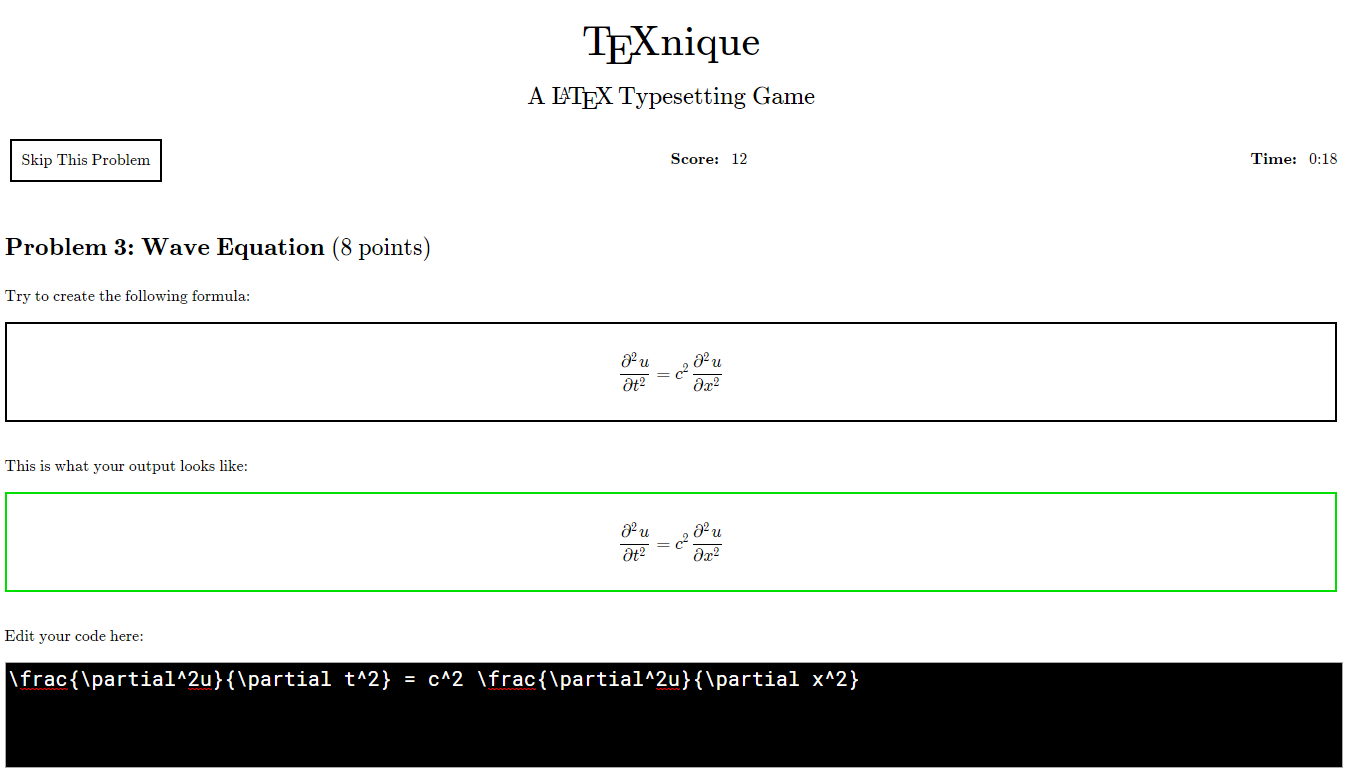
\includegraphics[width=1.0\linewidth,frame=]{./graphics/texnique.png}

% Caption is defined with a short and long version. The short version is shown in the 
% List of Figures section, and the long version is used directly with the figure. 			
	\caption[A screenshot of TeXnique, a game about typesetting equations.]{TeXnique, a game about typesetting equations \cite{texnique}. (Top) The game presents you with a rendered equation, (Bottom) the task is to enter LaTeX code that produces the same rendered equation. The green border on the lower rendering indicates it is a valid solution.}
	
% For figures label should be defined after the caption to ensure proper figure numbering.
	\label{fig:texnique}
\end{figure}
		
		TeXnique \cite{texnique} is web-browser based game for practising how to typeset equations in LaTeX. The game will present you with a rendered equation and your task is to type LaTeX code into the box below it such that your code produces the same (or closely matching / pixel equivalent) rendered equation. Figure \ref{fig:texnique} shows the game during play, the bottom rendered equation is bordered in green to indicate it is a valid match with the target. 

		% An example of how to center a passage of text, control local fontsize, 
		% and create a properly formatted and clickable URL.
		\begin{center}
		{\small \url{https://texnique.xyz}}
		\end{center}
		
		This is one of the more painful parts of typesetting a document, so it really takes a special kind of sadism to come up with such a game. Least to say, graduate students and researchers can be an odd bunch, and when we found this it was surprisingly addictive to compete over. 
		
		
		
	\section{Figures}
	\label{sec:typesetting_figures}
	
	In this template figures are numbered starting with the current chapter number followed by a figure number that resets to 1 each new chapter. As you can see below, the first figure is labelled Figure \ref{fig:dragon} because we are in Chapter \ref{chap:typesetting}.
	
	Figures in LaTeX are defined using a \lstinline|\begin{figure}...\end{figure}| environment and often immediately begin rendering in centre aligned mode by calling \lstinline|\centering|. Listing \ref{lst:latex_figure} below shows the LaTeX code used to typeset figure \ref{fig:dragon}. Figures \ref{fig:example_2x1} and \ref{fig:example_2x2} are defined similarly and make additional use of the \lstinline|\subfloat| command to position multiple images within a single figure environment, each with their own automatically incremented labels and individual captions.

	\lstinputlisting[label={lst:latex_figure}, caption={An example LaTeX excerpt demonstrating how to typeset figure \ref{fig:dragon} with a simple caption.}]{./listings/example_figure.tex}

	\subsection{Consistent presentation throughout the document}
		Figures work best in a document when you use a consistent style for formatting and captioning them and make sure that figures always actively support the content of the main text. 
	
	\subsection{Justified use of space in the document}
		All figures must be referred to directly in the main text of the document and discussed with meaningful and in depth critical analysis. If you don't need to use the figure to leverage and support your discussion then it is just taking up space and padding out the document. For example, you can use a command like \lstinline|\ref{fig:dragon}| to automatically get the figure number for Figure \ref{fig:dragon}. 	
		
		\begin{figure}[H]
	% [H] means put the figure HERE, directly when you input this code.
	\centering

	% We set the width of the figure based on the width of one line 
	% of text on the page. The value can be tuned to any value in 
	% [0.0, 1.0] to scale the image while maintaining its aspect ratio.
	\includegraphics[width=1.0\linewidth]{./graphics/dragon.png}
	
	% Caption is defined with a short and long version. The short 
	% version is shown in the List of Figures section, and the long 
	% version is used directly with the figure. 		
	\caption[Short caption.]{Long caption and citation \cite{whittle15_dragons}.}
	
	% For figures, \label should be defined after the caption to ensure 
	% proper figure numbering.
	\label{fig:dragon}
\end{figure}
		
	\subsection{Placement that supports and enhances the flow of the document}
		All figures shown in your document should be displayed in relevant locations, ideally just after that have been alluded to in the main text. Although there are many times where it is best to force a figure to the top or bottom of a nearby page.
	
	\subsection{Avoid directly importing other peoples images}
		You should avoid using other peoples figures whenever possible, and instead create your own figures for visualizing the specific methods and data you are working with in a way directly relevant to your project. 
	
	\subsection{Format sub-figures in LaTeX, not in the image itself}
		Construct sub-figures from multiple image files in LaTeX not in the image file itself. This allows you to tweak the positioning and layout without having to modify the images. It also allows for automatic formatting and numbering of captions and sub-captions. Figures \ref{fig:example_2x1} and \ref{fig:example_2x2} show examples of side-by-side and quad layouts respectively.
		
		% [H] means put the figure HERE, directly when you input this code.
\begin{figure}[H]
	\centering
	
% We use a figure width of 48.5% of the width of one line of text on 
% the page so there is some space between the images.
	\subfloat[Left image sub-caption.]{
		\includegraphics[width=0.485\linewidth]{./graphics/dragon.png}\label{fig:example_2x1_a}
	}~ % Use a tilde to add spacing for sub-figures that are displayed next to one another horizontally.
	\subfloat[Right image sub-caption.]{
		\includegraphics[width=0.485\linewidth]{./graphics/dragon.png}\label{fig:example_2x1_b}
	}\\ % New line before caption.

% Caption is defined with a short and long version. The short version is shown in the 
% List of Figures section, and the long version is used directly with the figure. 	
	\caption[A demonstration of a 2x1 sub-figure layout.]{Construct sub-figures from multiple image files in LaTeX not in the image file itself. This allows you to tweak the positioning and layout without having to modify the images. It also allows for automatic formatting and numbering of captions and sub-captions. Image of glass dragons rendered using Path Tracing \cite{whittle15_dragons}.}
	
% For figures label should be defined after the caption to ensure proper figure numbering.
	\label{fig:example_2x1}
	
\end{figure}
		
		% [H] means put the figure HERE, directly when you input this code.
\begin{figure}[H]
	\centering
	
% We use a figure width of 48.5% of the width of one line of text on 
% the page so there is some space between the images.
	\subfloat[Top-Left image sub-caption.]{
		\includegraphics[width=0.485\linewidth]{./graphics/dragon.png}\label{fig:example_2x2_a}
	}~ % Use a tilde to add spacing for sub-figures that are displayed next to one another horizontally.
	\subfloat[Top-Right image sub-caption.]{
		\includegraphics[width=0.485\linewidth]{./graphics/dragon.png}\label{fig:example_2x2_b}
	}\\ % New line before caption.
	\subfloat[Bottom-Left image sub-caption.]{
		\includegraphics[width=0.485\linewidth]{./graphics/dragon.png}\label{fig:example_2x2_c}
	}~ % Use a tilde to add spacing for sub-figures that are displayed next to one another horizontally.
	\subfloat[Bottom-Right image sub-caption.]{
		\includegraphics[width=0.485\linewidth]{./graphics/dragon.png}\label{fig:example_2x2_d}
	}\\ % New line before caption.
		
% Caption is defined with a short and long version. The short version is shown in the 
% List of Figures section, and the long version is used directly with the figure. 	
	\caption[A demonstration of a 2x2 sub-figure layout.]{A demonstration of a 2x2 sub-figure layout. Between A-B and C-D we use tilde symbols and between B-C we use a new line. Image of glass dragons rendered using Path Tracing \cite{whittle15_dragons}.}
	
% For figures label should be defined after the caption to ensure proper figure numbering.
	\label{fig:example_2x2}
	
\end{figure}
	
	\subsection{Robust captions that can stand in isolation}
		Figures need to be captioned such that they can be viewed in isolation and still be meaningful to the viewer. There will likely be some duplication of information that is written in the main text, but this is intended. 
	
	\subsection{Proper attribution and citation of images}
		\label{sec:typesetting_figures_citation}
		
		If an image does not belong to you it \textbf{must} be cited directly in the figure caption. \textbf{It is not correct to put a URL in the figure caption directly.} A URL in isolation is not an accurate or reliable way of directing a future reader to the exact content you are referencing. Instead make a new entry in your \lstinline|citations.bib| file and then reference that citation in the caption using the \lstinline|\cite{key}| command. Figures \ref{fig:dragon}, \ref{fig:example_2x1}, and \ref{fig:example_2x2} each include a statement in the caption stating ``Image of glass dragons rendered using Path Tracing \cite{whittle15_dragons}.''. When adding the BibTeX entry, try to find the proper information about the original author and source document to strengthen the citation in case the URL changes. 
	
	\section{Code Listings}
	\label{sec:typesetting_listings}
	
	Code listings should be formatted in the same style as figures and inline equations. It is important to use a monospace font so that characters line up vertically. Syntax highlighting is also extremely important for effectively displaying complicated code segments. To format inline code listings you can use the \lstinline[mathescape]|\lstinline$|$the_code$|$| command\footnote{So meta.}.
	
	% Longform Code listings should live in a code file, not embedded directly into your LaTeX code!
	\lstinputlisting[language={c}, label={lst:c_hello_world}, caption={An implementation of an important algorithm from our work.}]{./listings/hello_world.c}
	
	In LaTeX the ``Listings'' package can be used to properly format code and provide basic syntax highlighting, line numbering, and captioning of embedded code excerpts. Listing \ref{lst:listings} shows examples of how to properly format code using the listings package. 
	
	\newpage
	
	% Longform Code listings should live in a code file, not embedded directly into your LaTeX code!
	\lstinputlisting[label={lst:listings}, caption={Examples of methods for typesetting code listings within a LaTeX document.}]{./listings/listings.tex}
	
	\section{Tables}
	\label{sec:typesetting_tables}
	
	Tables are also quite predictably captioned and formatted the same way. It is important to decide on a style for how you will organize your data and apply that style consistently for all of your tables. Table \ref{tbl:example_table} shows one possible way of styling your data but is by no means the only way of doing so neatly. Consistency is the key. 
	
	% It's often a good idea to generate the LaTeX code for tables (python script or similar) so that if you rerun your code you don't have to typeset your results again by hand!
\begin{table}[H]
	\centering
	\scriptsize
	\caption[A demonstration of a table typeset in LaTeX.]{An example of a table formatted with caption.}
	
	% Tune the following two values that are being multiplied by the variable \textwidth
	% to control how large the scale of the table is, and how much is is squashed back 
	% to the final size.	
	\resizebox{0.8\textwidth}{!}{
		\begin{tabularx}{0.46\textwidth}{c|c|c|c|c|c}
			\toprule
			Some & Relevant & Fields & From & Your & Data\\
			\midrule
			0 & 0 & 0 & 0 & 0 & 0\\
			1 & 1 & 1 & 1 & 1 & 1\\
			2 & 2 & 2 & 2 & 2 & 2\\
			\bottomrule
		\end{tabularx}
		\label{tbl:example_table}
	}
\end{table}




	

	\chapter{Conclusions and Future Work}
\label{chap:conclusion}

In this document we have demonstrated the use of a LaTeX thesis template which can produce a professional looking academic document. 

\section{Contributions} 
\label{sec:conclusion_contributions}

The main contributions of this work can be summarized as follows:
\begin{description}	

	\item[$\bullet$ A LaTeX thesis template]\hfill
	
	Modify this document by adding additional top level content chapters. These descriptions should take a more retrospective tone as you include summary of performance or viability. 
	
	
	\item[$\bullet$ A typesetting guide of useful primitive elements]\hfill
	
	Use the building blocks within this template to typeset each part of your document. Aim to use simple and reusable elements to keep your document neat and consistently styled throughout.
	
	\item[$\bullet$ A review of how to find and cite external resources]\hfill
		
	We review techniques and resources for finding and properly citing resources from the prior academic literature and from online resources. 
	
\end{description}

\section{Future Work}
\label{sec:conclusion_future_work}

Future editions of this template may include additional references to Futurama.
	
% Formatting citations properly when they are rendering incorrectly in your PDF can be fiddly,
% espectially when punctuation and international characters are involed. Sometimes multiple re-compilations
% are needed in addition to clearing temporary auxiliary files to see your changes in your document.
% Insert the bibliography using citations contained in the file citations.bib
	\bibintoc%
	\bibliography{citations} 
	
% In the appendix you might include a full code listing for an implemented algorithm that you showed a 
% small chunk of in one of your chapters. If you have extra graphs for ablation style experiments you 
% might enumerate them within the appendix and use \label{name} and \ref{name} to automatically insert 
% the correct section locations when you talk about them in your chapters.
% Within appendix.tex you should use chapters as the top level section dividers.
	\appendix
	\addappheadtotoc
	\chapter{Implementation of a Relevant Algorithm}
\label{app:implementation_algorithm}

% Code listings should live in a code file, not embedded directly into your LaTeX code!
\lstinputlisting[language=c, label={lst:c_hello_world}, caption={An implementation of an important algorithm from our work.}]{./listings/hello_world.c}

\chapter{Supplementary Data}
\label{app:supplementary_data}

The results of large ablative studies can often take up a lot of space, even with neat visualization and formatting. Consider putting full results in an appendix chapter and showing excerpts of interesting results in your chapters with detailed analysis. You can use labels and references to refer the reader here for the full data.

	
\end{document}